\chapter{Initial Setup}

TACC has a full-fledged double entry General Ledger (GL) and chart of
accounts system that allows for finely tuned reporting and tracking of
customer billing.  Before TACC can be used fully the General Ledger and
Chart of Accounts must be carefully planned and defined within the
system.  This can be accomplished in the following steps:

\begin{enumerate}
\item Plan the accounts you wish TACC to use.  The standard accounts
that TACC will use by default are:
\begin{itemize}
\item Asset
\item Liabilities \& Equity
\item Income
\item Cost of Goods Sold
\item Selling Expenses
\item Administrative Expenses
\item Other Income and Expense
\end{itemize}
TACC places no restrictions on how accounts are numbered or the number
of accounts that you can have.  These are used strictly for reporting
purposes.  To access the account types, click on the \emph{Admin Menu}, then
\emph{Other Lists}, then \emph{Accounts}.  This will bring up the
\emph{Chart of Accounts} window (Figure ~\ref{fig:ChartOfAccounts} on
page ~\pageref{fig:ChartOfAccounts}).

\label{QuickStartAccountTypes}
Configuring the Account Types is done through the \emph{Options} menu
and selecting \emph{Account Types}.  From the Account Types window, you
can add, edit and delete the types of accounts that will appear in the
Chart of Accounts.
\begin{figure}[hbtp]
\center{ \fbox{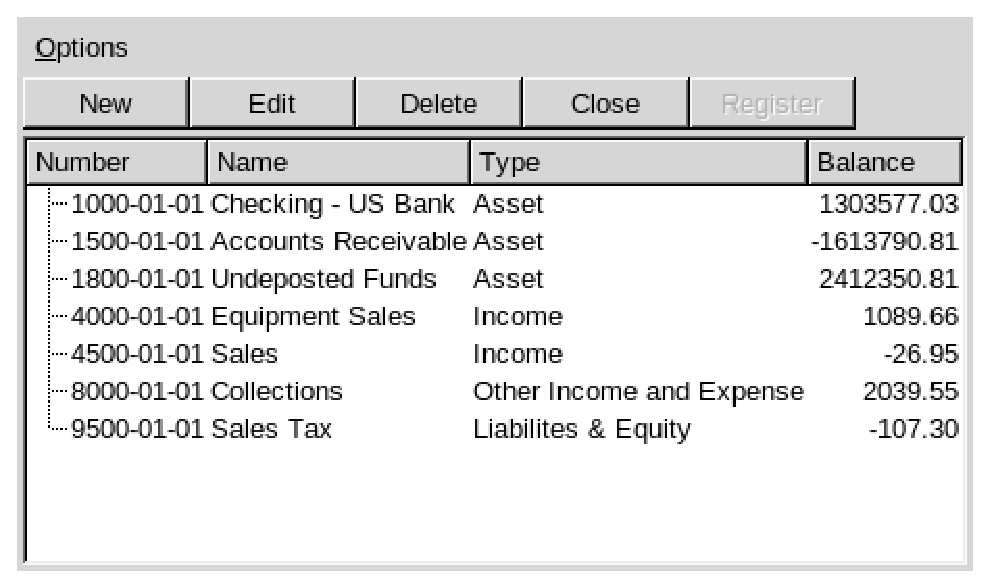
\includegraphics[width=7cm]{figures/ChartOfAccounts.eps}} }
\caption{ \label{fig:ChartOfAccounts} Chart of Accounts}
\end{figure}
\item Create the accounts that you will use.  TACC will need at a
minimum the following accounts defined:
\begin{description}
\item[Cash/Checking] This account holds payments after they have been
processed.
\item[Accounts Receivable] This is where TACC tracks a customer's
billables.
\item[Sales] This is where TACC tracks services that are sold to customers.
\item[Undeposted Funds] When check payments are received they are put
into this account until they are deposted, at which time they are
usually transferred to the \emph{Cash/Checking} account.
\item[Collections] When accounts are sent to collection, the balance is
transferred from \emph{Accounts Receivable} to this account.
\end{description}
This is what TACC requires at a minimum to function.  There is no upper
limit on how many accounts can be defined within TACC.  For more details
on the Chart of Accounts, see the \emph{Chart of Accounts} section on
page ~\pageref{Chart of Accounts}.
\item After defining your accounts, you must configure TACC to use them.
This is done in the \emph{Accounting} area in the \emph{Settings}
section of TACC accessed from the \emph{Admin} menu (see Figure
~\ref{fig:SettingsAccounting} on page ~\pageref{fig:SettingsAccounting}).
\begin{figure}[hbtp]
\center{ \fbox{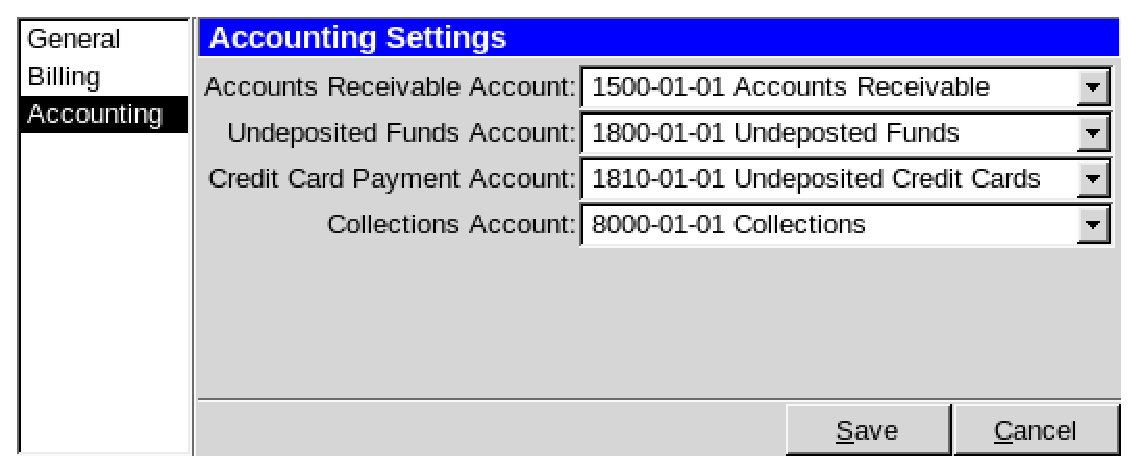
\includegraphics[width=8cm]{figures/SettingsAccounting.eps}} }
\caption{ \label{fig:SettingsAccounting} Accounting Settings}
\end{figure}
For each item, choose the account you have created from the Chart of
Accounts.  When you are finished, hit \emph{Save}.
\item Configure Billables to be tracked in the one or more Sales
accounts.  Each Billable Item in TACC can be assigned a different
account to post to in the Chart of Accounts.  They are configured
individually in the Billable Items section accessed from the
\emph{Admin} menu, then \emph{Other Lists} then \emph{Billable Items}
(see Figure ~\ref{fig:BillableItems} on page
~\pageref{fig:BillableItems}).
\begin{figure}[hbtp]
\center{ \fbox{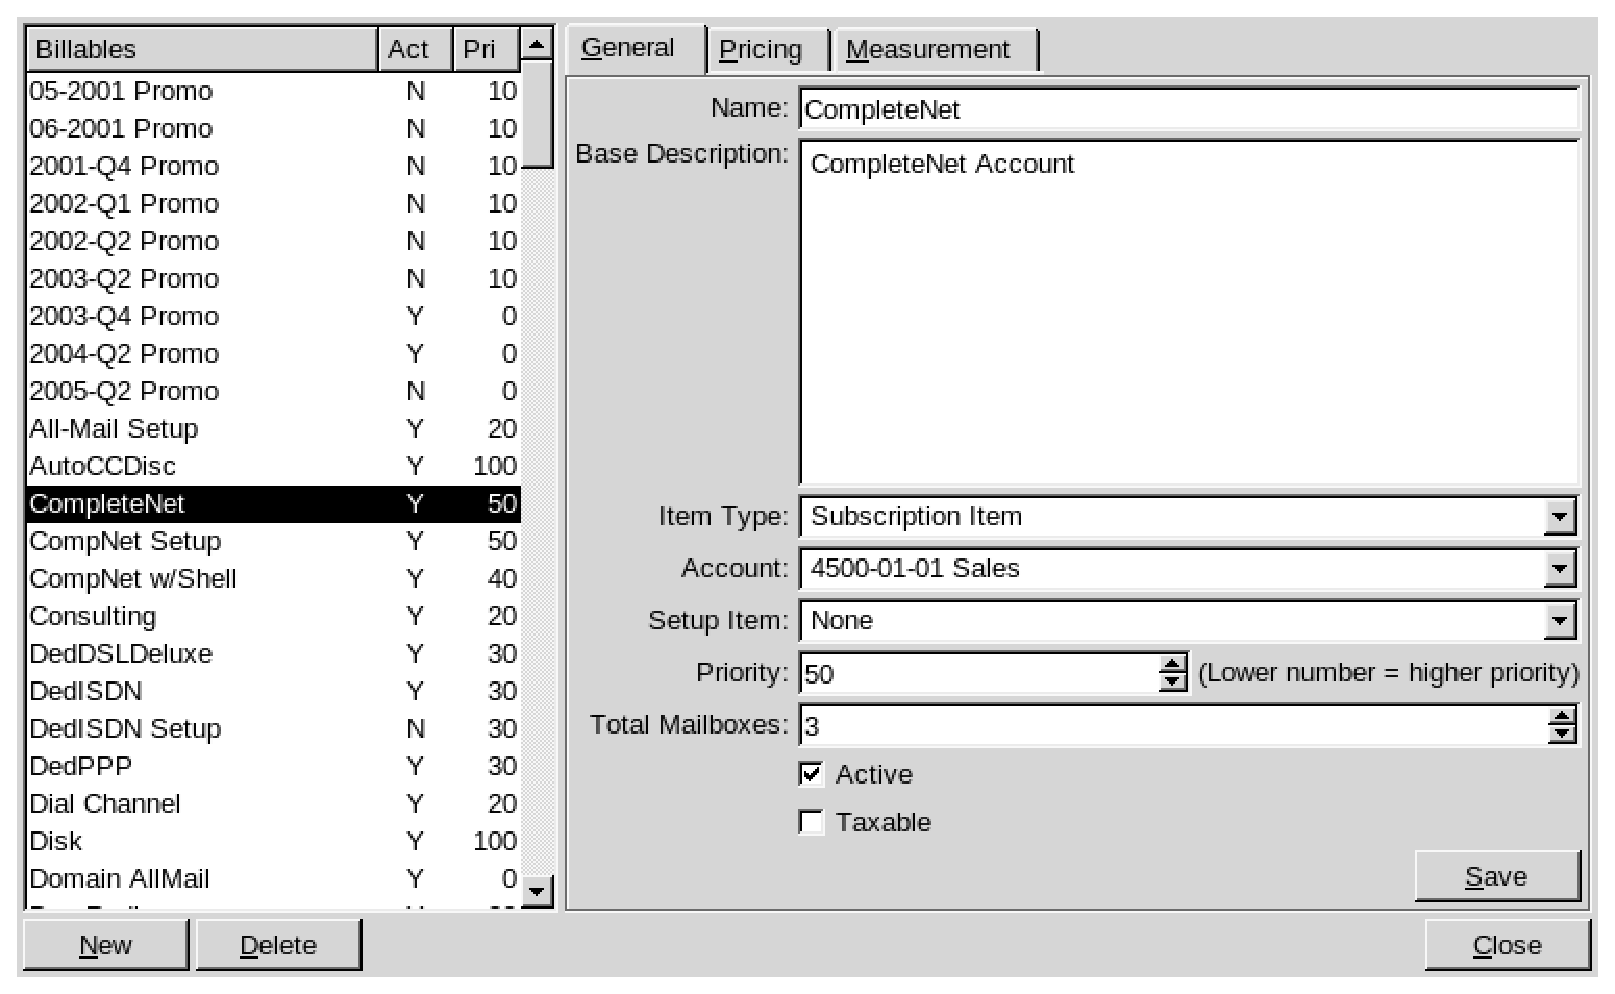
\includegraphics[width=12cm]{figures/BillableItems.eps}} }
\caption{ \label{fig:BillableItems} Billable Items}
\end{figure}
Each Billable Item has an \emph{Account} field that associates the
billable with an entry in the Chart of Accounts.  Each time a customer
is charged for this billable item, it will post to the account specified
here and the \emph{Accounts Recievable} account specified in
Settings.  There is no default, so each billable item will need to be
configured individually.
\item Configure Packages to be tracked in one or more sales accounts.
Packages encapsulate a group of billable items to be billed as a single
charge to a customer.  Because a package contains a group of billable
items that may post to different accounts, they must be configured
seperately from the individual billable items.  To access the list of
Packages, use the \emph{Admin} menu, then \emph{Other Lists} then
\emph{Package Editor} (see Figure ~\ref{fig:PackagesList} on page
~\pageref{fig:PackagesList}).
\begin{figure}[hbtp]
\center{ \fbox{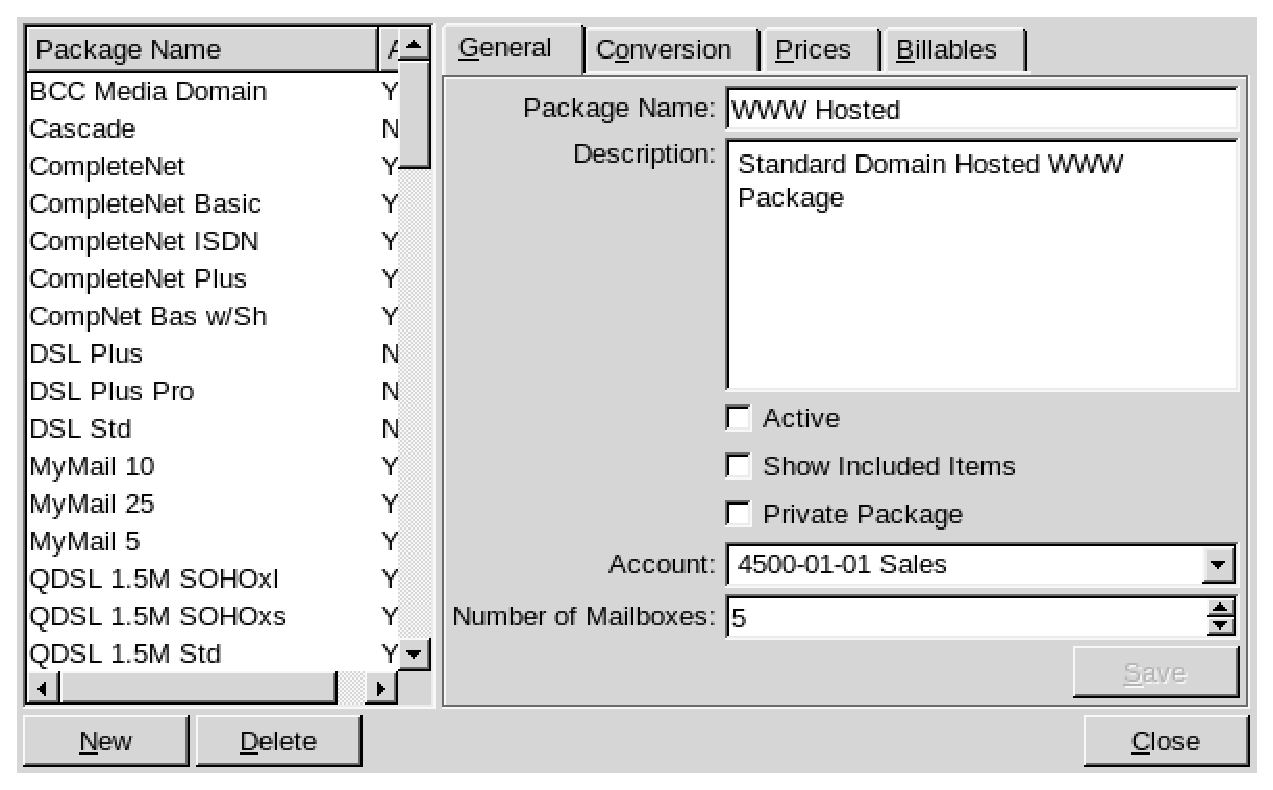
\includegraphics[width=12cm]{figures/PackagesList.eps}} }
\caption{ \label{fig:PackagesList} Packages List}
\end{figure}
Very similar to the Billable Items, the account must be associated with
the package.  Each time a customer is billed with this pacakge, it will
post to the account specified here.
\end{enumerate}
After these steps have been completed, TACC will be able to accurately
track and generate reports from the General Ledger.

\section{Chart of Accounts}
\label{Chart of Accounts}
The Chart of Accounts determines how sales and other financial reports
are generated from within TACC.  Each account in the Chart of Accounts
must be of the specific type laid out in the Account Types (see page
~\pageref{QuickStartAccountTypes}) and have an Account Number associated
with it.

Account Numbers should be grouped together within a numerical range for
a specific type of account.  For example, all accounts that are
\emph{Assets} are normally found in the range 1000-1999, \emph{Income}
accounts are normally 3000-3999, etc.  You can have duplicate account
numbers within TACC, but they will be treated as individual items.
{\bf It his highly recommended that you make all account numbers unique}.

Account Numbers are free-form within TACC and do not actually have to
specify a number.  TACC employs a "mask" that determines how the account
numbers must be entered and will be displayed.  If you wanted to
extended TACC to use an 8 digit account number, with the first four
digits being the standard accounting account number, the next two being
the company, and the final two being the location (which is the default
setting), you would use a mask to do this.

The default mask is {\tt D999-99-99}, where "D" is a digit between 1 and 9,
and "9" is any digit between 0 and 9.  The dashes are automatically used
and inserted.  For information on changing the account mask and the
possible values, please see the \it{TACC Administrators Guide}.

